% Provenance (never printed): see sources/outline_sources.md (Year 1: litho-, bio- and
% chronostratigraphy; boundary stratotypes; mass extinctions as global markers; the
% international chart). Exercise and problem values in the Book 3 scratch calculator
% calc/ch24.py; the chart from figdata/bachelor-1/ics_chart.py (shared ics rows).
% The principles of relative dating, eras and periods are Book 1's (g7 geological-time) and
% are re-founded here. Mass extinctions belong to the biology series (recalled in prose);
% their Earth causes are the Year 2 volume's (phanerozoic-earth). Correlation of logs and
% unconformities are ch. 5's; facies ch. 21's; compaction ch. 23's. Radiometric dating is
% ch. 25's. Sequence stratigraphy, facies models and Walther's law are the Year 3 volume's;
% magnetostratigraphy too: prose pointers only. "Transgression" is explained in prose.
\chapter{स्तरिक पैमाना}\label{ch:b1:stratigraphic-scale}

इटज़ुरुन के समुद्र-तट पर, बास्क तट पर ज़ुमाइया में, चट्टानें चूना-पत्थर और मार्ल की पतली परतों से बनी हैं, जो झुकी हुई हैं और सैकड़ों मीटर तक दोहराई गई हैं। एक \omterm{def:b1:geological-maps:geological-map}{संपर्क} पर, जहाँ एक पीला चूना-पत्थर का संस्तर खत्म होता है और लाल मार्ल शुरू होते हैं, चट्टान में चार अक्षरों वाली एक कांस्य-तश्तरी जड़ी है (नीचे का चित्र)। यह एक स्वर्ण-स्पाइक है। वह पूरे ग्रह के लिए भूवैज्ञानिक समय के एक विभाजन --- सेलैंडियन \omterm{def:b1:stratigraphic-scale:chronostratigraphy}{चरण} --- के आरंभ का क्षण तय करता है। पैटागोनिया या साइबेरिया की कोई चट्टान सेलैंडियन है, यदि वह उस \omterm{def:b1:geological-maps:geological-map}{संपर्क} पर दर्ज क्षण के बाद, और पैमाने पर ऊपर के अगले स्पाइक पर दर्ज क्षण से पहले, जमी। यह अध्याय समझाता है कि भूवैज्ञानिकों को ऐसे चिह्न की आवश्यकता क्यों पड़ी: चट्टानों के ढेर को बाँटने के तीन अलग तरीके, उन्हें क्रम देने वाले सिद्धांत, दूर-दूर के खंडों को जोड़ने वाली रेखाएँ, और वह अंतर्राष्ट्रीय चार्ट जो परिणाम को समेटता है।

\begin{omfigure}
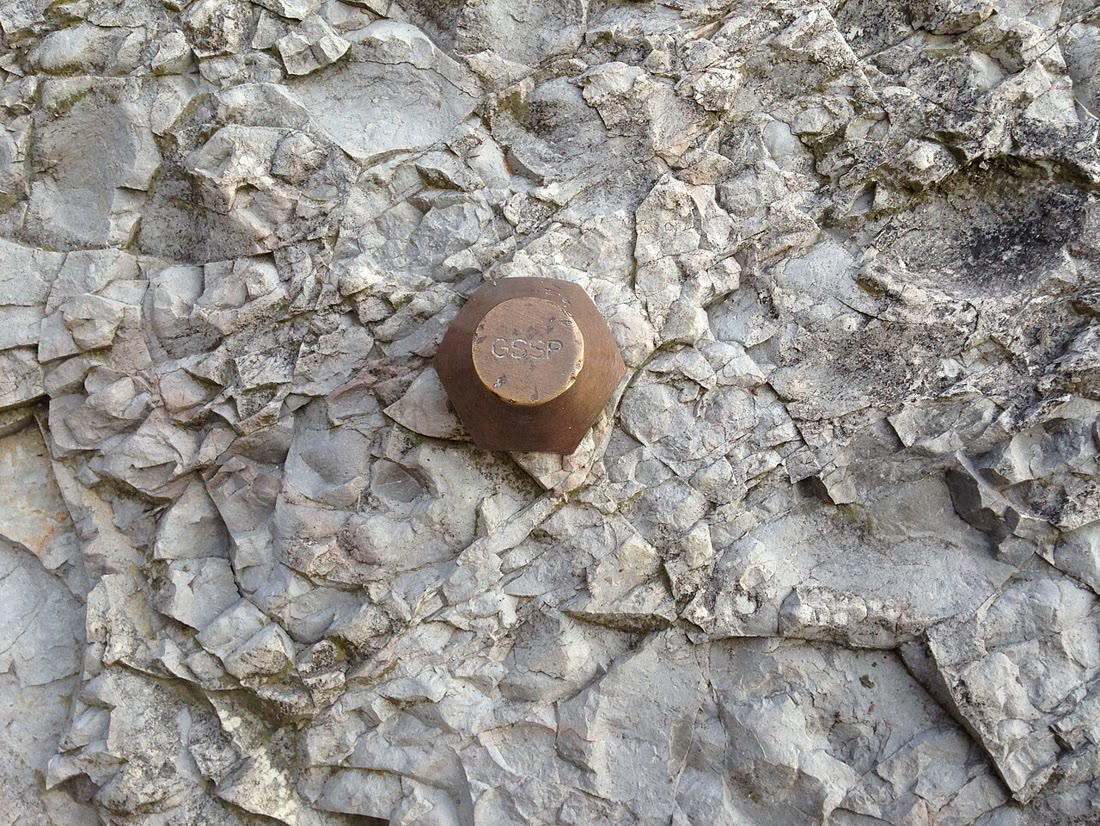
\includegraphics[width=0.62\linewidth]{images/book3/b1-golden-spike-zumaia.jpg}

{\small ज़ुमाइया खंड में सेलैंडियन \omterm{def:b1:stratigraphic-scale:chronostratigraphy}{चरण} का स्वर्ण-स्पाइक: कांस्य का एक मार्कर, जिस पर \omterm{def:b1:stratigraphic-scale:gssp}{GSSP} अंकित है, एक \omterm{def:b1:stratigraphic-scale:lithostratigraphy}{संरचना} के सबसे ऊपरी चूना-पत्थर संस्तर के शीर्ष पर, अगली \omterm{def:b1:stratigraphic-scale:lithostratigraphy}{संरचना} की लाल मार्ल के आधार पर लगा हुआ। (फ़ोटो: Josugoni, CC~BY-SA~4.0, विकिमीडिया कॉमन्स के माध्यम से।)}
\label{fig:b1:stratigraphic-scale:zumaia}
\end{omfigure}
% ledger: commons:zumaia-gssp, gssp:selandian

\begin{recall}
एक ढेर में, जो उलटा न गया हो, हर परत अपने नीचे की परत से नई होती है; चट्टानों को काटने वाली कोई \omterm{def:b1:stratigraphic-scale:lithostratigraphy}{संरचना} उनसे नई होती है; जीवाश्म पुरानी परतों से नई परतों की ओर हर जगह एक ही क्रम में बदलते हैं; और पृथ्वी का इतिहास युगों और भूवैज्ञानिक कालों में बँटा है, जिनमें से हर एक के आरंभ की आयु वर्षों में है, और जो एक अंतर्राष्ट्रीय चार्ट में संकलित हैं (पुस्तक~1, कक्षा~7)। एक बोरहोल-लॉग गहराई के विरुद्ध मिली इकाइयाँ दर्ज करता है, और सहसंबंध एक लॉग से दूसरे लॉग तक एक ही इकाइयों का मिलान करता है (\cref{def:b1:cross-sections:log}); एक \omterm{def:b1:cross-sections:unconformity}{असंगति} अपरदन या अनिक्षेपण का एक पृष्ठ है (\cref{def:b1:cross-sections:unconformity})। एक अवसादी संस्तर-पिंड वह चट्टान का पिंड है जिसके लक्षण उसके निक्षेपण के परिवेश का अभिलेख रखते हैं (\cref{def:b1:clastic-sediments:facies})। जीव-विज्ञान की पुस्तकें वर्णन करती हैं कि प्रजातियाँ कैसे प्रकट होती हैं और विलुप्त होती हैं, और वे कुछ सामूहिक विलोपन, जिनमें थोड़े समय में सभी प्रजातियों का बड़ा भाग लुप्त हो गया।
\end{recall}

\section{चट्टानों को बाँटने के तीन तरीके}\label{sec:b1:stratigraphic-scale:three}

एक भूवैज्ञानिक जो एक चट्टान का लॉग बनाता है, उसी परतों के ढेर को तीन तरीकों से बाँट सकता है: उसकी बनावट से, उसमें मिलने वाले जीवाश्मों से, और उस समय से जिसमें वे जमी थीं। तीनों विभाजन अलग-अलग प्रश्नों के उत्तर देते हैं, और उनकी सीमाएँ एक-दूसरे से मेल खाना ज़रूरी नहीं। किसी इकाई को नाम देने और परिभाषित करने के नियम अंतर्राष्ट्रीय समझौते से तय होते हैं।
% ledger: isg:lithostratigraphy

\begin{definition}[संरचना, सदस्य, समूह]\label{def:b1:stratigraphic-scale:lithostratigraphy}
एक \emph{अश्मस्तरिक इकाई}\index{अश्मस्तरिक इकाई} चट्टान का एक पिंड है जिसे उसकी बनावट और दूसरे पिंडों के बीच उसकी स्थिति से परिभाषित और पहचाना जाता है, उसकी आयु चाहे जो हो। मुख्य इकाई \emph{संरचना}\index{संरचना (अश्मस्तरिक)} है: चट्टान का एक पिंड, जो अपने पड़ोसियों से इतना भिन्न हो कि क्षेत्र के पैमाने पर मानचित्रित किया जा सके, और जिसमें पूरा स्तंभ बाँटा जाना चाहिए। एक \emph{सदस्य}\index{सदस्य (अश्मस्तरिक)} संरचना का एक नामित उपविभाग है, जो अपनी बनावट से पहचाना जाता है; एक \emph{समूह}\index{समूह (अश्मस्तरिक)} दो या अधिक संरचनाओं का अनुक्रम है जिनमें महत्त्वपूर्ण बनावटी लक्षण साझा हैं। एक औपचारिक नाम स्थानीय भौगोलिक नाम को पद या प्रमुख चट्टान से जोड़ता है: केल बलुआ पत्थर, मार्डन शेल संरचना।
\end{definition}
% ledger: isg:lithostratigraphy

एक \omterm{def:b1:stratigraphic-scale:lithostratigraphy}{संरचना} एक मीटर से कम या कई हज़ार मीटर मोटी हो सकती है। वह अपने प्रारूप खंड से केवल वहीं तक बढ़ाई जाती है जहाँ तक उसकी बनावट पहचानी जा सके, इसलिए उसकी सीमाएँ चट्टान का अनुसरण करती हैं, समय का नहीं।
% ledger: isg:lithostratigraphy

\begin{definition}[जैव-क्षेत्र, सूचक जीवाश्म, पहली उपस्थिति का आँकड़ा]\label{def:b1:stratigraphic-scale:biozone}
एक \emph{जैव-क्षेत्र}\index{जैव-क्षेत्र} स्तरों का एक पिंड है जो उनमें मिलने वाले जीवाश्मों से परिभाषित या अभिलक्षित होता है। एक \emph{परास-क्षेत्र}\index{परास-क्षेत्र} किसी एक टैक्सन की ज्ञात उपस्थितियाँ रखता है; एक \emph{अंतराल-क्षेत्र}\index{अंतराल-क्षेत्र} दो निर्दिष्ट जीवाश्म-क्षितिजों के बीच के स्तरों का पिंड है, उदाहरण के लिए दो टैक्सा की सबसे निचली उपस्थितियाँ। किसी टैक्सन की \emph{पहली उपस्थिति का आँकड़ा}\index{पहली उपस्थिति का आँकड़ा} (FAD) उसकी सबसे निचली उपस्थिति का क्षितिज है, और \emph{अंतिम उपस्थिति का आँकड़ा}\index{अंतिम उपस्थिति का आँकड़ा} उसकी सबसे ऊँची का। एक \emph{सूचक जीवाश्म}\index{सूचक जीवाश्म} एक टैक्सन है जिससे जैव-क्षेत्र पहचाना जाता है: सबसे अच्छे व्यापक, प्रचुर, आसानी से पहचाने जाने वाले और अल्पजीवी होते हैं।
\end{definition}
% ledger: isg:biostratigraphy, og:stratigraphy-principles

एक जीवाश्म क्षितिज की कोई मोटाई नहीं होती; एक \omterm{def:b1:stratigraphic-scale:biozone}{जैव-क्षेत्र} कुछ मीटर या कुछ सौ मीटर मोटा हो सकता है, यह इस पर निर्भर करता है कि जब वे टैक्सा जिए तब तलछट कितनी तेज़ी से जमा हुआ। चूँकि प्रजातियाँ विकसित होती हैं और विलुप्त होने के बाद कभी दोबारा नहीं आतीं, किसी एक आयु का समुदाय अनूठा होता है। कुछ सबसे अच्छे \omterm{def:b1:stratigraphic-scale:biozone}{सूचक जीवाश्म} सूक्ष्मजीवाश्म हैं, जैसे फ़ोरामिनिफ़ेरा और कोनोडॉन्ट: व्यापक, प्रचुर, और इतने छोटे कि किसी कुएँ की कटिंग से निकाले जा सकें।
% ledger: isg:biostratigraphy, og:stratigraphy-principles

\begin{definition}[कालस्तरिक और भूकालिक इकाइयाँ]\label{def:b1:stratigraphic-scale:chronostratigraphy}
एक \emph{कालस्तरिक इकाई}\index{कालस्तरिक इकाई} भूवैज्ञानिक समय के किसी दिए गए अंतराल में बनी सभी चट्टानों का पिंड है, और केवल उसी में; उसकी सीमाएँ समान-आयु के पृष्ठ हैं। वह समय-अंतराल स्वयं एक \emph{भूकालिक इकाई}\index{भूकालिक इकाई} है। पदानुक्रम, सबसे छोटे से, ये हैं: \emph{चरण}\index{चरण (कालस्तरिक)} (उसका समय: एक आयु), \emph{श्रेणी}\index{श्रेणी (कालस्तरिक)} (एक युग), \emph{तंत्र}\index{तंत्र (कालस्तरिक)} (एक काल), इरेथेम (एक महायुग) और ईओनोथेम (एक महाकल्प); हर इकाई नीचे की पदानुक्रम की कई क्रमिक इकाइयों से बनी होती है।
\end{definition}
% ledger: isg:chronostratigraphy

ये दोनों शब्द एक ही विभाजन को चट्टान या समय के रूप में देखते हैं (\cref{tab:b1:stratigraphic-scale:ranks}): जुरासिक \omterm{def:b1:stratigraphic-scale:chronostratigraphy}{तंत्र} की चट्टानें जुरासिक काल में जमीं, और निम्न जुरासिक \omterm{def:b1:stratigraphic-scale:chronostratigraphy}{श्रेणी} प्रारंभिक जुरासिक युग में। \omterm{def:b1:stratigraphic-scale:chronostratigraphy}{चरण} पूरी दुनिया में पहचानी जाने वाली सबसे छोटी इकाई है।
% ledger: isg:chronostratigraphy, chart:danian

\begin{table}[htbp]
\centering
\begin{tabular}{lll}
\hline
\omterm{def:b1:stratigraphic-scale:chronostratigraphy}{कालस्तरिक इकाई} (चट्टान) & \omterm{def:b1:stratigraphic-scale:chronostratigraphy}{भूकालिक इकाई} (समय) & उदाहरण \\
\hline
ईओनोथेम & महाकल्प & फ़ैनेरोज़ोइक \\
इरेथेम & महायुग & सेनोज़ोइक \\
\omterm{def:b1:stratigraphic-scale:chronostratigraphy}{तंत्र} & काल & पैलियोजीन \\
\omterm{def:b1:stratigraphic-scale:chronostratigraphy}{श्रेणी} & युग & पैलियोसीन \\
\omterm{def:b1:stratigraphic-scale:chronostratigraphy}{चरण} & आयु & डेनियन (\qtyrange{66.00}{61.66}{\Ma}) \\
\hline
\end{tabular}
\caption{कालस्तरिक और भूकालिक इकाइयों की पदानुक्रमी श्रेणियाँ, उन इकाइयों के साथ जो सेनोज़ोइक के पहले \omterm{def:b1:stratigraphic-scale:chronostratigraphy}{चरण}, डेनियन, को समाहित करती हैं।}
\label{tab:b1:stratigraphic-scale:ranks}
\end{table}
% ledger: isg:chronostratigraphy, chart:danian

\section{सिद्धांत और सहसंबंध}\label{sec:b1:stratigraphic-scale:principles}

चट्टानों की आयु वर्षों में तय होने से पहले, घटनाओं का क्रम स्वयं चट्टानों से पढ़ा गया। स्तरिकी के मूल सिद्धांत 1669 में निकोलस स्टेनो ने प्रस्तुत किए; 1785 और 1800 के बीच हटन और विलियम स्मिथ ने परतों को समय के अंतरालों के रूप में, और उनके जीवाश्मों को उन्हें पहचानने के लिए, उपयोग में जोड़ा।
% ledger: og:stratigraphy-principles, usgs:hutton-smith

\begin{definition}[स्तरिकी के सिद्धांत]\label{def:b1:stratigraphic-scale:principles}
\begin{enumerate}
  \item \emph{अध्यारोपण का सिद्धांत}\index{अध्यारोपण का सिद्धांत}: अवसादी परतों के एक अनुक्रम में, जो उलटा न गया हो, हर परत उस परत से नई है जिस पर वह टिकी है।
  \item \emph{मूल क्षैतिजता का सिद्धांत}\index{मूल क्षैतिजता का सिद्धांत}: तलछट और लावा-प्रवाह क्षैतिज रूप से, या लगभग इसी प्रकार जमते हैं --- एक द्रोणी के किनारों पर थोड़े ढलान के साथ।
  \item \emph{पार्श्व सातत्य का सिद्धांत}\index{पार्श्व सातत्य का सिद्धांत}: एक द्रोणी के भीतर एक परत हर दिशा में निरंतर फैलती है, जब तक वह द्रोणी के किनारे पर, या किसी बाधा के सामने, पतली न हो जाए; घाटी द्वारा कटी परत दूसरी ओर जारी रहती है।
  \item \emph{आर-पार संबंधों का सिद्धांत}\index{आर-पार संबंधों का सिद्धांत}: एक पिंड या \omterm{def:b1:stratigraphic-scale:lithostratigraphy}{संरचना} जो चट्टानों को काटती है --- एक डाइक, एक भ्रंश, एक अपरदन-पृष्ठ --- उन चट्टानों से नई है जिन्हें वह काटती है।
  \item \emph{जीव-जातीय अनुक्रम का सिद्धांत}\index{जीव-जातीय अनुक्रम का सिद्धांत}: जीवाश्म टैक्सा हर क्षेत्र में एक ही क्रम में एक-दूसरे का स्थान लेते हैं, इसलिए जिन चट्टानों में एक ही समुदाय है वे एक ही आयु की हैं।
\end{enumerate}
\end{definition}
% ledger: og:stratigraphy-principles, eli:relative-dating, usgs:fossil-succession, isg:chronostratigraphy

सिद्धांत समान रूप से प्रबल नहीं हैं। अध्यारोपण एक ऐसा क्रम देता है जिसका हर दूसरी विधि को सम्मान करना होगा। मूल क्षैतिजता वह है जो एक झुकी परत को बाद के विरूपण का अभिलेख बनाती है। पार्श्व सातत्य वह है जो एक भूवैज्ञानिक को एक घाटी के दोनों ओर एक ही परत खींचने देता है, और, एक सीमित दूरी के भीतर, ज़मीन पर खींचा गया एक परत-तल वहाँ समान आयु की सबसे अच्छी रेखा है। जीव-जातीय अनुक्रम वह है जो महासागरों को पार करता है; वह अगले अनुच्छेदों का विषय है।
% ledger: isg:chronostratigraphy, og:stratigraphy-principles

\subsection*{जैव-क्षेत्रों द्वारा सहसंबंध}

जीवाश्मों द्वारा सहसंबंध दो खंडों में पहली और अंतिम उपस्थितियों के क्रम की तुलना करता है (नीचे का चित्र)। दोनों समान रूप से विश्वसनीय नहीं हैं। किसी खंड में मिले किसी टैक्सन का सबसे ऊँचा जीवाश्म इस पर निर्भर करता है कि कितने संरक्षित हुए: जहाँ वे दुर्लभ हैं, वहाँ पाया गया अंतिम जीवाश्म उस स्तर से कहीं नीचे हो सकता है जिस पर वह टैक्सन सचमुच विलुप्त हुआ, और अपरदित होकर दोबारा जमा जीवाश्म उसके ऊपर दिख सकता है। पहली उपस्थिति भी विस्थापित हो सकती है, पर एक व्यापक टैक्सन जो तेज़ी से फैला, वह द्रोणी भर में लगभग एक ही स्तर पर पहुँचता है।
% ledger: isg:biostratigraphy

\begin{omfigure}
\begin{tikzpicture}[font=\footnotesize, y=0.13cm]
  % section 1: 40 m, sandstone 0-14, shale 14-40
  \fill[lith sandstone] (0,0) rectangle (0.8,14);
  \fill[lith shale] (0,14) rectangle (0.8,40);
  \draw[black!70] (0,0) rectangle (0.8,40);
  \node[anchor=south, font=\small] at (1.4,41.5) {खंड 1};
  \foreach \x/\a/\b/\t in {1.1/0/27/a, 1.4/10/34/b, 1.7/20/40/c, 2.0/30/40/d} {
    \draw[line width=2.2pt, omThm] (\x,\a) -- (\x,\b);
    \node[anchor=base, font=\scriptsize] at (\x,-4.5) {\t};
  }
  \foreach \y/\z in {5/a, 15/b, 25/c, 35/d}
    \node[anchor=east, font=\scriptsize] at (-0.1,\y) {क्षेत्र \z};
  \foreach \y in {10,20,30} \draw[black!50] (-1.3,\y) -- (0,\y);
  % scale bar
  \draw[thick] (-1.5,0) -- (-1.5,10) node[midway, anchor=east, font=\scriptsize] {\qty{10}{m}};
  % section 2: 24 m, sandstone 0-3, shale 3-24
  \begin{scope}[xshift=7cm]
    \fill[lith sandstone] (0,0) rectangle (0.8,3);
    \fill[lith shale] (0,3) rectangle (0.8,24);
    \draw[black!70] (0,0) rectangle (0.8,24);
    \node[anchor=south, font=\small] at (1.4,25.5) {खंड 2};
    \foreach \x/\a/\b/\t in {1.1/0/13/a, 1.4/6/20/b, 1.7/12/24/c, 2.0/18/24/d} {
      \draw[line width=2.2pt, omThm] (\x,\a) -- (\x,\b);
      \node[anchor=base, font=\scriptsize] at (\x,-4.5) {\t};
    }
    \foreach \y/\z in {3/a, 9/b, 15/c, 21/d}
      \node[anchor=west, font=\scriptsize] at (2.3,\y) {क्षेत्र \z};
    \foreach \y in {6,12,18} \draw[black!50] (0.8,\y) -- (2.3,\y);
  \end{scope}
  % correlation of the first appearances
  \foreach \u/\v/\t in {10/6/b, 20/12/c, 30/18/d}
    \draw[densely dashed, omThm!70!black] (2.15,\u) -- (6.85,\v)
      node[pos=0.5, fill=white, inner sep=1pt, font=\scriptsize] {FAD \t};
\end{tikzpicture}

{\small परास-चार्ट और जैव-क्षेत्रों द्वारा सहसंबंध (काल्पनिक टैक्सा \emph{a} से \emph{d} तक)। मोटी पट्टियाँ हर खंड में टैक्सा के परास हैं। तीन \omterm{def:b1:stratigraphic-scale:biozone}{अंतराल-क्षेत्र} \emph{b}, \emph{c} और \emph{d} की पहली उपस्थितियों से सीमित हैं, जो खंड-दर-खंड जोड़ी गई हैं (धराशायी)। \emph{a} की अंतिम उपस्थिति खंड 1 में क्षेत्र~\emph{c} के ऊपरी भाग में, और खंड 2 में उसके आधार के पास पड़ती है: वह एक कमज़ोर मार्गदर्शक है। क्षेत्र खंड 2 में पतले हैं, जहाँ तलछट धीमी दर से जमा हुआ।}
\label{fig:b1:stratigraphic-scale:range-chart}
\end{omfigure}

\begin{method}[जैव-क्षेत्रों से खंडों का सहसंबंध]\label{met:b1:stratigraphic-scale:biozones}
\begin{enumerate}
  \item हर खंड के लिए, हर टैक्सन का परास ऊँचाई के विरुद्ध आलेखित कीजिए: उसकी सबसे निचली से सबसे ऊँची उपस्थिति तक।
  \item वे जीवाश्म-क्षितिज चुनिए जो क्षेत्रों को परिभाषित करते हैं --- प्राथमिकता से व्यापक टैक्सा की पहली उपस्थितियाँ, जो संस्तर-प्रकार से स्वतंत्र हों।
  \item इन क्षितिजों पर हर खंड में क्षेत्र-सीमाएँ खींचिए।
  \item वही क्षितिज खंड-दर-खंड जोड़िए; जाँचिए कि रेखाएँ एक-दूसरे को न काटें, जैसा अध्यारोपण माँगता है।
  \item दो रेखाओं के बीच हर खंड में हर क्षेत्र की मोटाई पढ़िए; जहाँ कोई क्षेत्र न हो, वहाँ एक \omterm{def:b1:cross-sections:unconformity}{असंगति} या संस्तर-प्रकार का बदलाव खोजिए, इससे पहले कि यह निष्कर्ष निकालें कि टैक्सन अनुपस्थित है।
\end{enumerate}
\end{method}

जैव-स्तरिक सहसंबंध तभी अच्छा है जब उसके जीवाश्म परिवेश से स्वतंत्र हों। केवल रेतीले तटों पर रहने वाला एक द्विकपाटी केवल बलुआ पत्थरों में मिलता है; उसका खंड-दर-खंड अनुसरण बलुआ पत्थर का अनुसरण करता है, समय का नहीं। जैव-स्तरिक सहसंबंध इसलिए आवश्यक रूप से काल-सहसंबंध नहीं है: वह एक ऐसी \omterm{def:b1:stratigraphic-scale:lithostratigraphy}{संरचना} का अनुसरण कर सकता है जिसकी आयु स्थान-स्थान पर बदलती है।
% ledger: isg:biostratigraphy

\subsection*{ऐसी सीमाएँ जो समय को पार करती हैं}

एक ही समय पर अलग-अलग स्थानों पर अलग-अलग तलछट जमते हैं: तट पर रेत, तट से दूर कीचड़, और बालू से वंचित मंच पर उससे भी आगे चूना। इसलिए समान आयु की एक रेखा एक शैल-प्रकार से दूसरे में गुज़रती है। इसके विपरीत, द्रोणी के पार खींची गई एक शैल-विज्ञानी सीमा सभी स्थानों पर समान आयु की रेखा होना आवश्यक नहीं।
% ledger: og:stratigraphy-principles, isg:chronostratigraphy

\begin{definition}[तिर्यक्-कालिक सीमा]\label{def:b1:stratigraphic-scale:diachronous}
एक सीमा \emph{तिर्यक्-कालिक}\index{तिर्यक्-कालिक सीमा} होती है जब उसकी आयु उसके साथ-साथ स्थान-स्थान पर बदलती है। संरचनाओं और संस्तरों की सीमाएँ प्रायः तिर्यक्-कालिक होती हैं; कालस्तरिक इकाइयों की सीमाएँ परिभाषा से नहीं होतीं।
\end{definition}
% ledger: isg:lithostratigraphy, isg:chronostratigraphy, isg:biostratigraphy

सबसे क्लासिक मामला एक ट्रांसग्रेशन है: \omterm{def:b1:diagenesis-basins:eustasy}{सापेक्ष समुद्र-स्तर} इतनी तेज़ी से उठता है कि तलछट बनी जगह को भर नहीं पाता, और तट भूमि की ओर खिसकता है। समुद्र-तट की बालू हर क्षण तट पर जमती है, इसलिए बलुआ पत्थर की एक चादर उसके साथ अंदर की ओर फैलती है; समुद्र की ओर की कीचड़ उसके ऊपर आती है। बलुआ पत्थर का ऊपरी भाग तब खिसकती तट-रेखा का निशान है: भूमि की ओर युवा, समुद्र की ओर पुराना (नीचे का चित्र)। एक ऊर्ध्वाधर खंड में देखा गया संस्तरों का क्रम --- शेल के नीचे बलुआ पत्थर, चूना-पत्थर के नीचे शेल --- एक ही क्षण में मंच के आर-पार उनके क्रम को दोहराता है; पुस्तक~5 इसी को अपने संस्तर-प्रतिरूपों का आधार बनाती है।
% ledger: og:stratigraphy-principles, isg:lithostratigraphy

\begin{omfigure}
\begin{tikzpicture}[font=\footnotesize, x=1cm, y=1cm]
  % basement surface B(x) = 1.6 (1 - x/14), rising towards the land on the left
  \fill[lith granite] (0,-0.5) -- (0,1.6) -- (14,0) -- (14,-0.5) -- cycle;
  \fill[lith sandstone] (0,1.6) -- (14,0) -- (14,0.5) -- (0,2.1) -- cycle;
  \fill[lith shale] (0,2.1) -- (14,0.5) -- (14,1.5) -- (0,3.1) -- cycle;
  \fill[lith limestone] (0,3.1) -- (14,1.5) -- (14,3.6) -- (0,3.6) -- cycle;
  \draw[unconformity] (0,1.6) -- (14,0);
  \draw[black!70] (0,2.1) -- (14,0.5) (0,3.1) -- (14,1.5);
  \draw[black!70] (0,-0.5) rectangle (14,3.6);
  % time lines: horizontal, from the basement (or the left edge) to the right edge
  \foreach \y/\t in {0.6/1, 1.1/2, 1.6/3, 2.1/4, 2.6/5, 3.1/6} {
    \pgfmathsetmacro{\xs}{max(0, 14*(1-\y/1.6))}
    \draw[omThm, thick, densely dashed] (\xs,\y) -- (14,\y) node[anchor=west, text=black] {$t_\t$};
  }
  % two sections
  \foreach \x/\n in {3/1, 11/2} {
    \draw[very thick, black] (\x,-0.5) -- (\x,3.6);
    \node[anchor=south, font=\small] at (\x,3.65) {खंड \n};
  }
  \node[fill=white, inner sep=1pt, font=\scriptsize] at (5.6,1.21) {बलुआ पत्थर};
  \node[fill=white, inner sep=1pt] at (12.6,1.2) {शेल};
  \node[fill=white, inner sep=1pt] at (7.0,3.25) {चूना-पत्थर};
  \node[fill=white, inner sep=1pt] at (12.0,-0.25) {आधार-तल};
  \draw[-{Stealth}, thick] (5.6,4.35) -- (3.6,4.35) node[anchor=east] {भूमि};
  \draw[-{Stealth}, thick] (8.4,4.35) -- (10.4,4.35) node[anchor=west] {समुद्र};
\end{tikzpicture}

{\small ट्रांसग्रेशन के दौरान जमी बलुआ पत्थर की एक चादर (योजनाबद्ध, ऊर्ध्वाधर पैमाना बढ़ाकर)। धराशायी रेखाएँ $t_1$ से $t_6$ तक समान आयु के बिंदुओं को जोड़ती हैं, $t_1$ सबसे पुराना। जहाँ एक आधार-तल से मिलती है, वह अपने समय की तट-रेखा पर शुरू होती है; समुद्र की ओर वह रेत से कीचड़ में बदलती है और, युवतर में, चूने में। बलुआ पत्थर का ऊपरी भाग खंड~2 में $t_1$ और $t_2$ के बीच है, पर खंड~1 में $t_3$ और $t_4$ के बीच: \omterm{def:b1:stratigraphic-scale:lithostratigraphy}{संरचना} की सीमा तिर्यक-कालिक है, भूमि की ओर युवा।}
\label{fig:b1:stratigraphic-scale:diachronous}
\end{omfigure}

तट के साथ सीमा की आयु कितनी तेज़ी से बदलती है? एक तटीय मैदान पर, जो भूमि की ओर धीरे उठता है, उत्तर ज्यामिति का विषय है।

\begin{proposition}[ट्रांसग्रेशन की गति]\label{prop:b1:stratigraphic-scale:transgression}
एक तटीय मैदान एकसमान ढलान $s$ से भूमि की ओर उठता है, और \omterm{def:b1:diagenesis-basins:eustasy}{सापेक्ष समुद्र-स्तर} स्थिर दर $R$ से उठता है, तट पर कोई तलछट जोड़े बिना। तब तट-रेखा इस गति से भूमि की ओर बढ़ती है
\[
  u = \frac{R}{s},
\]
और तट-रेखा का अनुसरण करने वाली सीमा, भूमि में दूरी $d$ और आगे के एक बिंदु पर, $\Delta t = d/u = d\,s/R$ से युवा है।
\end{proposition}

\begin{proof}
माना $x$ एक स्थिर बिंदु से भूमि के भीतर की दूरी है और $z$ ऊँचाई; मैदान रेखा $z = s x$ है, और समय $t$ पर समुद्र की सतह $z = z_0 + R t$ है। तट-रेखा वहाँ है जहाँ वे मिलते हैं: $s\,x(t) = z_0 + R t$, इसलिए $x(t) = (z_0 + R t)/s$ और $\mathrm dx/\mathrm dt = R/s$। तट-रेखा भूमि में दूरी $d$ पर एक बिंदु तक समय $d/u = d\,s/R$ के बाद पहुँचती है।
\end{proof}

अनुपात इसलिए बड़ा है क्योंकि तटीय मैदान लगभग समतल होते हैं। प्रति दस लाख वर्ष \qty{10}{m} की वृद्धि, जो $1$ में $2000$ ढलान वाले मैदान पर हो, तट को प्रति दस लाख वर्ष \qty{20}{km} भूमि की ओर खिसकाती है; तब चट्टान-दीवार में जो बलुआ पत्थर का ऊपरी भाग एक ही सतह जैसा दिखता है, वह भूमि में \qty{20}{km} दूर दस लाख वर्ष छोटा है। तट तक लाया गया तलछट ट्रांसग्रेशन को धीमा करता है या उसे उलट देता है।

\subsection*{समान आयु की रेखाएँ}

तो फिर समय का सहसंबंध क्या करता है, यदि बनावट नहीं करती और जीवाश्म केवल लगभग? सबसे अच्छी रेखाएँ उन घटनाओं से बनती हैं जो एक साथ हर जगह निशान छोड़ती हैं। एक ज्वालामुखीय राख एक विस्तृत क्षेत्र पर उस चीज़ में गिरती है जो भूवैज्ञानिक रूप से एक क्षण है, और रेत, कीचड़ और चूने पर समान रूप से बैठ जाती है: राख-परत संस्तर-सीमाओं को पार करने वाली समान आयु की रेखा है, और उसे अक्सर \cref{ch:b1:radiometric-methods} की विधियों से वर्षों में आँका जा सकता है। पृथ्वी के चुंबकीय क्षेत्र के उत्क्रमण, जिन्हें पुस्तक~5 में लिया गया है, कई प्रकार की चट्टानों में दर्ज होते हैं और उनका क्रम ज्ञात होने पर विश्वभर में पहचाने जा सकते हैं; कार्बन समस्थानिकों में अचानक बदलाव भी ऐसे ही हैं, जैसा वह जो येप्रेसियन के आधार को चिह्नित करता है (\cref{tab:b1:stratigraphic-scale:gssps})। दो आँके गए स्तरों के बीच किसी भी परत की आयु इस धारणा से आँकी जाती है कि तलछट स्थिर दर से जमा हुआ।
% ledger: isg:chronostratigraphy

\begin{proposition}[दो आँके गए स्तरों के बीच आयु]\label{prop:b1:stratigraphic-scale:interpolation}
एक सतत खंड की दो परतों की, ऊँचाइयाँ $z_1 < z_2$, आयु $t_1 > t_2$ हैं। यदि उनके बीच तलछट स्थिर दर से जमा हुआ, तो उनके बीच ऊँचाई $z$ के एक स्तर की आयु
\[
  t = t_1 - f\,(t_1 - t_2), \qquad f = \frac{z - z_1}{z_2 - z_1},
\]
और संचय की दर $r = (z_2 - z_1)/(t_1 - t_2)$ है। यदि दोनों आयुओं की स्वतंत्र मानक अनिश्चितताएँ $\sigma_1$ और $\sigma_2$ हैं, तो प्रक्षेपित आयु की अनिश्चितता
\[
  \sigma_t = \sqrt{(1 - f)^2 \sigma_1^2 + f^2 \sigma_2^2}.
\]
\end{proposition}

\begin{proof}
प्रति स्थिर दर $r$ पर ऊँचाई समय के साथ रैखिक बढ़ती है: $z - z_1 = r\,(t_1
- t)$, क्योंकि आयु ऊपर की ओर घटती है। $z_2$ पर, $z_2 - z_1 = r\,(t_1 - t_2)$ है, जो $r$ देता है; दोनों संबंधों को भाग देने पर $t_1 - t = f\,(t_1 - t_2)$ मिलता है। आयु दो स्वतंत्र राशियों का रैखिक संयोजन है, $t = (1 - f)\,t_1 + f\,t_2$; $a X + b Y$ का प्रसरण, स्वतंत्र $X$ और $Y$ के लिए, $a^2
\operatorname{Var} X + b^2 \operatorname{Var} Y$ है, जो $\sigma_t$ देता है।
\end{proof}

अनिश्चितता दो आँके गए संस्तरों के बीच सबसे छोटी है और वहाँ $\sigma_1$ और $\sigma_2$ के बड़े से कभी बड़ी नहीं होती। वास्तविक सीमा धारणा है: तलछट स्पंदों में जमता है, छिपे हुए विरामों पर रुक सकता है, और रेत और कीचड़ में अलग-अलग संपीड़ित होता है (\cref{prop:b1:diagenesis-basins:solid}), इसलिए प्रक्षेपित आयु खंड की नियमितता से बेहतर नहीं है।

\section{सीमा-स्ट्रैटोटाइप}\label{sec:b1:stratigraphic-scale:gssp}

एक \omterm{def:b1:stratigraphic-scale:chronostratigraphy}{कालस्तरिक इकाई} चट्टान में परिभाषित होती है, उसकी आयु तय होने से पहले। पुरानी प्रथा हर \omterm{def:b1:stratigraphic-scale:chronostratigraphy}{चरण} को पूरी इकाई के एक प्रारूप खंड से वर्णित करती थी; पर एक प्रारूप खंड का ऊपरी भाग और अगले का निचला भाग, अलग-अलग स्थानों पर चुने गए, उनके बीच अनिर्दिष्ट समय का अंतर छोड़ सकते थे या उनमें अतिव्यापन हो सकता था। आधुनिक प्रथा हर इकाई की केवल निचली सीमा को एक खंड के एक बिंदु पर परिभाषित करती है; ऊपरी सीमा अगली इकाई की निचली सीमा है। तब कोई समय-अंतराल दो इकाइयों के बीच न गिर सकता है, न दोनों का हो सकता है।
% ledger: isg:stratotype, isg:chronostratigraphy

\begin{definition}[सीमा स्ट्रैटोटाइप, इकाई स्ट्रैटोटाइप, GSSP]\label{def:b1:stratigraphic-scale:gssp}
एक \emph{स्ट्रैटोटाइप}\index{स्ट्रैटोटाइप} चट्टान का नामित खंड है जो किसी इकाई या सीमा के संदर्भ का मानक है। एक \emph{इकाई स्ट्रैटोटाइप}\index{इकाई स्ट्रैटोटाइप} पूरी इकाई का प्रारूप खंड है; एक \emph{सीमा स्ट्रैटोटाइप}\index{सीमा स्ट्रैटोटाइप} वह खंड है जिसमें दो इकाइयों के बीच की सीमा को परिभाषित करने वाला विशिष्ट बिंदु है। एक \emph{वैश्विक सीमा स्ट्रैटोटाइप खंड और बिंदु}\index{वैश्विक सीमा स्ट्रैटोटाइप खंड और बिंदु (GSSP)} (GSSP) अंतर्राष्ट्रीय कालस्तरिक पैमाने की एक इकाई की सीमा स्ट्रैटोटाइप है: एक खंड में एक ही बिंदु, अंतर्राष्ट्रीय समझौते से चुना गया, जो एक \omterm{def:b1:stratigraphic-scale:chronostratigraphy}{चरण} के आधार को, और उससे आरंभ होने वाली हर बड़ी इकाई के आधार को, परिभाषित करता है।
\end{definition}
% ledger: isg:stratotype, isg:chronostratigraphy, gssp:protocol

\omterm{def:b1:stratigraphic-scale:gssp}{GSSP} चट्टान में एक बिंदु है, आयु नहीं। उसकी आयु वर्षों में वही है जो उस बिंदु का सर्वोत्तम आयु-निर्धारण देता है, और वह बिंदु को हिलाए बिना परिष्कृत की जा सकती है। खंड इस प्रकार चुना जाता है कि बिंदु कहीं और खोजा जा सके: सीमा के आर-पार निक्षेपण निरंतर हो (कभी अपरदन-पृष्ठ पर नहीं, जहाँ लुप्त समय सीमा को अस्पष्ट बना देता), प्राथमिकता समुद्री हो, व्यापक वर्गों के अच्छी तरह संरक्षित जीवाश्मों से समृद्ध, उस स्तर पर संस्तर-प्रकार में परिवर्तन के बिना, थोड़ा विकृत या बदला हुआ, सुलभ और सुरक्षित। सबसे ऊपर, बिंदु एक चुने हुए संकेत से मेल खाने वाले स्तर पर रखा जाता है --- आमतौर पर किसी टैक्सन की पहली उपस्थिति --- अन्य संकेतों (राख-परतें, चुंबकीय उत्क्रमण, समस्थानिक परिवर्तन) से समृद्ध एक अंतराल के भीतर, जिनसे वह स्तर दूर से पहचाना जा सके। एक स्थायी चिह्न, स्वर्ण-स्पाइक, बिंदु पर लगाया जाता है।
% ledger: isg:chronostratigraphy, isg:stratotype, gssp:protocol

\begin{inthefield}[सीमा कैसे चुनी जाती है]
एक सीमा का अध्ययन उस उपआयोग के एक कार्यदल द्वारा होता है जो \omterm{def:b1:stratigraphic-scale:chronostratigraphy}{तंत्र} के लिए उत्तरदायी है; वह उम्मीदवार खंडों की तुलना करता है, उन्हें परत-दर-परत लॉग करता है, उनके जीवाश्म, राख-परतें और समस्थानिक नमूने लेता है, और एक प्रस्ताव लिखता है। प्रस्ताव को \qty{60}{\%} से अधिक का महा-बहुमत चाहिए --- उपआयोग के लगभग बीस विशेषज्ञ मतदाताओं का --- फिर वह अंतर्राष्ट्रीय कालस्तरिक आयोग के मतदान सदस्यों, उसके कार्यकारी अधिकारियों और उसके सत्रह उपआयोगों के अध्यक्षों के पास जाता है, और अंत में भूवैज्ञानिक विज्ञान के अंतर्राष्ट्रीय संघ की कार्यकारी समिति के पास, जिसकी स्वीकृति उसे पुष्ट करती है। परिणाम प्रकाशित होते हैं, चिह्न चट्टान में लगाया जाता है, और नई स्थापित सीमा में दस वर्षों तक कोई परिवर्तन प्रस्तावित नहीं किया जा सकता।
\end{inthefield}
% ledger: gssp:protocol

\begin{table}[htbp]
\centering
\small
\begin{tabular}{>{\raggedright\arraybackslash}p{2.4cm}>{\raggedright\arraybackslash}p{1.27cm}>{\raggedright\arraybackslash}p{3.7cm}>{\raggedright\arraybackslash}p{5.53cm}c}
\hline
आधार & आयु (\unit{\Ma}) & खंड & बिंदु का चिह्न & अनुमोदित \\
\hline
फ़ॉर्च्यूनियन (कैम्ब्रियन) & 538.8 & फ़ॉर्च्यून हेड, न्यूफ़ाउंडलैंड, कनाडा & \emph{ट्राइकोफ़ाइकस पेडम} की अनुरेखी जीवाश्म के रूप में पहली उपस्थिति & 1992 \\
लोचकोविअन (डेवोनियन) & 419.62 & क्लोंक, प्राग के निकट, चेक गणराज्य & ग्रैप्टोलाइट \emph{मोनोग्रैप्टस यूनिफ़ॉर्मिस} की पहली उपस्थिति & 1972 \\
इंडुअन (ट्राइऐसिक) & 251.902 & मेइ\-शान, झेजि\-यांग, चीन & कोनोडॉन्ट \emph{हिन्डियोडस पार्वस} की पहली उपस्थिति, परत 27c के आधार पर & 2001 \\
डेनियन (पैलियोजीन) & 66.00 & वेद जेरफ़ान, अल-केफ़, ट्यूनीशिया & \qty{50}{cm} गहरी काली सीमा-मृत्तिका का आधार; इरीडियम विसंगति & 1991 \\
सेलैंडियन & 61.66 & ज़ुमाइया, स्पेन & लाल मार्ल का आधार; एक नैनोजीवाश्म समूह का दूसरा विकिरण & 2008 \\
येप्रेसियन (इओसीन) & 56.00 & दबाबिया, लक्सर के निकट, मिस्र & एक कार्बन-समस्थानिक उछाल का आधार & 2003 \\
चिबानियन & 0.774 & चिबा, जापान & एक टेफ़्रा का आधार, एक चुंबकीय उत्क्रमण के ठीक नीचे & 2020 \\
मेघालयन & 0.0042 & मॉमलुह गुफ़ा, मेघालय, पूर्वोत्तर प्रदेश & एक स्पेलियोथेम में \qty{7.45}{mm} गहरा स्तर & 2018 \\
\hline
\end{tabular}
\caption{आठ \omterm{def:b1:stratigraphic-scale:gssp}{GSSP}। चिह्न हैं टैक्सों की पहली उपस्थितियाँ, एक भू-रासायनिक विसंगति, एक समस्थानिक उछाल, एक चुंबकीय उत्क्रमण, और एक गुफा-निक्षेप में दर्ज एक जलवायु घटना।}
\label{tab:b1:stratigraphic-scale:gssps}
\end{table}
% ledger: gssp:fortunian, gssp:lochkovian, gssp:induan, gssp:danian, gssp:selandian, gssp:ypresian, gssp:chibanian, gssp:meghalayan

\Cref{tab:b1:stratigraphic-scale:gssps} दिखाती है कि चुने गए संकेत कितने विविध हैं। तालिका की पैलियोज़ोइक और मेसोज़ोइक सीमाएँ जीवाश्मों की पहली उपस्थितियों पर टिकी हैं, एक ग्रैप्टोलाइट और एक कोनोडॉन्ट; कैम्ब्रियन के आधार पर जीवाश्म एक अनुरेखी जीवाश्म है, किसी जानवर की गतिविधि से तलछट में छोड़ा गया निशान, न कि स्वयं जानवर। सेनोज़ोइक उदाहरणों में संकेत रासायनिक और भौतिक हैं: डेनियन का इरीडियम, येप्रेसियन का कार्बन-समस्थानिक उछाल, और वह चुंबकीय उत्क्रमण जो चिबानियन बिंदु से \qty{1.1}{m} ऊपर है। तालिका की सबसे युवा सीमा समुद्री चट्टान में बिल्कुल नहीं है: मेघालयन का आधार एक स्पेलियोथेम के भीतर एक स्तर है, गुफा में उगा निक्षेप, जो \num{4200} वर्ष पहले की एक जलवायु घटना दर्ज करता है।
% ledger: gssp:fortunian, gssp:danian, gssp:ypresian, gssp:chibanian, gssp:meghalayan

\begin{dated}{2026}
% ledger: gssp:count, chart:stage-count
अक्टूबर 2026 में अंतर्राष्ट्रीय कालस्तरिक आयोग की तालिका में 80 अनुमोदित \omterm{def:b1:stratigraphic-scale:gssp}{GSSP} सूचीबद्ध थे, और दो और प्रस्तावित। पहला 1972 में क्लोंक पर अनुमोदित हुआ; सबसे हाल का 2024 में, जब सिलूरियन के दो सीमा-बिंदु, जो अब तक वेल्स में परिभाषित थे, स्पेन और चेक गणराज्य में नए खंडों में ले जाए गए। फ़ैनेरोज़ोइक के पैमाने के 101 चरणों में से 21 के पास अभी कोई अनुमोदित \omterm{def:b1:stratigraphic-scale:gssp}{GSSP} नहीं था; उनके आधार अनंतिम हैं।
\end{dated}

फ़ैनेरोज़ोइक से नीचे, पैमाना अधिकतर अलग तरह से बँटा है। अपने सबसे युवा \omterm{def:b1:stratigraphic-scale:chronostratigraphy}{तंत्र}, एडियाकरन, के अलावा, प्रीकैम्ब्रियन समझौते से चुनी गई गोल आयुओं पर कटा है --- ये विभाजन बिंदुओं से नहीं, वर्षों में परिभाषित हैं।
% ledger: isg:chronostratigraphy

\section{सामूहिक विलोपन चिह्नों के रूप में}\label{sec:b1:stratigraphic-scale:extinctions}

जीव-विज्ञान की पुस्तकें सामूहिक विलोपनों को उन क्षणों के रूप में वर्णित करती हैं जब भूवैज्ञानिक रूप से कम समय में प्रजातियों का बड़ा भाग लुप्त हो गया। स्तरिकी के लिए ऐसी घटना एक उपहार है: एक क्षितिज जो हर महाद्वीप और हर महासागर में मिलता है, जिसके आर-पार जीवाश्म समुदाय पूरी तरह बदल जाते हैं। उनमें से दो फ़ैनेरोज़ोइक के तीन महायुगों को सीमित करते हैं।
% ledger: schulte:kpg, burgess:end-permian

\subsection*{क्रिटेशियस का अंत}

1980 में अल्वारेज़, अल्वारेज़, असारो और मिशेल ने गहरे समुद्र के चूना-पत्थरों में इरीडियम मापा --- प्लैटिनम धातुओं में से एक, जो पृथ्वी की पपड़ी में ब्रह्मांड की उनकी प्रचुरता की तुलना में घटा हुआ है --- क्रिटेशियस और तृतीयक के बीच की सीमा के आर-पार, जो आज क्रिटेशियस और पैलियोजीन की सीमा है, K--Pg सीमा। उन्हें इटली में पृष्ठभूमि से लगभग 30 गुना, डेनमार्क में 160 गुना, और न्यूज़ीलैंड में 20 गुना समृद्ध मिला, ठीक विलोपनों के स्तर पर। उन्होंने प्रस्ताव रखा कि लगभग $\qty{10}{km}$ चौड़ा एक \omterm{def:b1:comparative-planetology:small-bodies}{क्षुद्रग्रह}, चार कम या अधिक, पृथ्वी से टकराया और अपने ही द्रव्यमान का लगभग 60 गुना पिसी हुई चट्टान वायुमंडल में फेंक दी; धूल विश्वभर में फैली और आसमान को अंधेरा कर दिया। सीमा की मृत्तिका, उन्होंने ध्यान दिलाया, ऊपर और नीचे के चूना-पत्थरों की मृत्तिका से रासायनिक रूप से भिन्न है।
% ledger: alvarez:iridium

बाद के काम ने सीमा को एक ही प्रभाव से जोड़ा, चिक्सुलब। आर्गन–आर्गन आयु-निर्धारण उस प्रभाव और विलोपनों वाली सीमा को एक-दूसरे के \num{32000} वर्षों के भीतर रखता है, और साक्ष्य की एक समीक्षा ने निष्कर्ष निकाला कि प्रभाव ने विलोपन शुरू किया; विलोपन उस समय में भी पड़ा जब दक्षिण एशिया में बेसाल्ट का एक विशाल उद्गार हुआ। डेनियन के आधार --- पैलियोजीन और पूरे सेनोज़ोइक का आधार --- का \omterm{def:b1:stratigraphic-scale:gssp}{GSSP} ट्यूनीशिया में अल-केफ़ के गहरे सीमा-मृत्तिका के आधार पर, इरीडियम विसंगति पर रखा गया है। वही सीमा भूमि पर, कोलोराडो में दिखती है (नीचे का चित्र)।
% ledger: renne:kpg, schulte:kpg, gssp:danian, commons:kt-tlsp

\begin{omfigure}
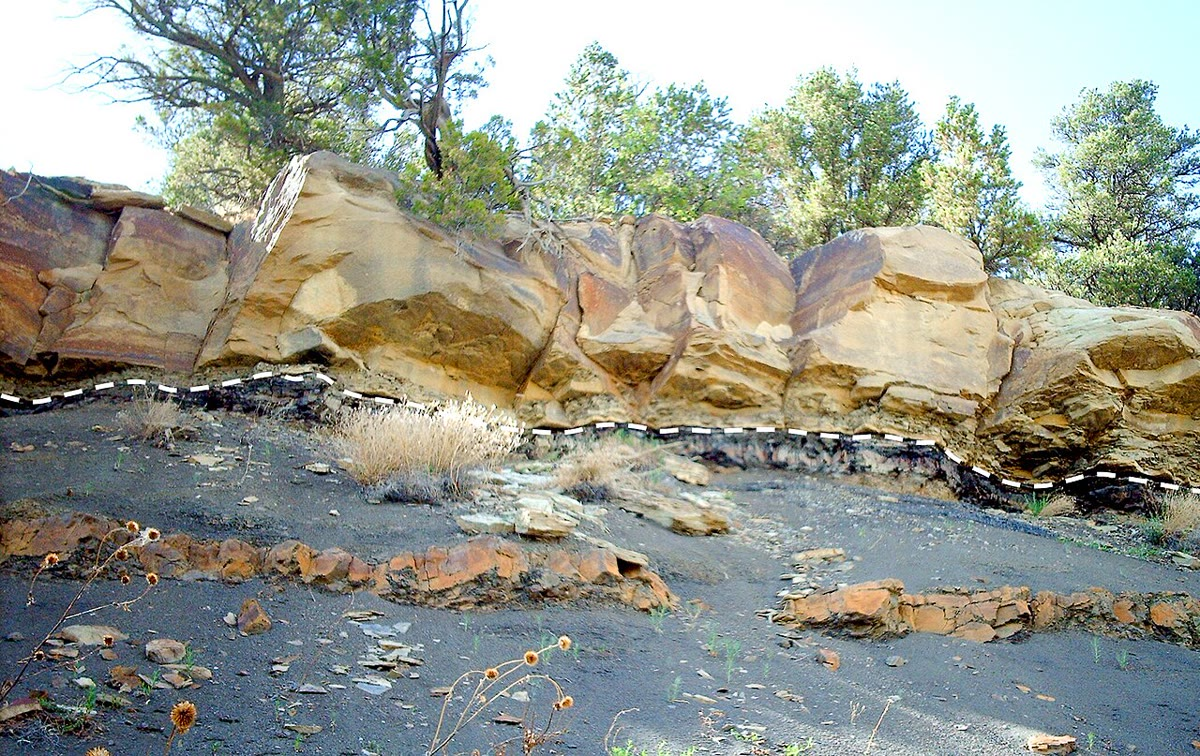
\includegraphics[width=0.78\linewidth]{images/book3/b1-kpg-boundary-trinidad.jpg}

{\small सीमा, क्रिटेशियस और पैलियोजीन के बीच, धराशायी रेखा से चिह्नित, ट्रिनिडैड लेक स्टेट पार्क, कोलोराडो में: ऊपर बलुआ पत्थर, नीचे और सीमा के साथ गहरे संस्तर। (फ़ोटो: Nationalparks, CC~BY-SA~2.5, विकिमीडिया कॉमन्स के माध्यम से; धराशायी रेखा मूल में है।)}
\label{fig:b1:stratigraphic-scale:kpg}
\end{omfigure}
% ledger: commons:kt-tlsp

\subsection*{पर्मियन का अंत}

पर्मियन के अंत का विलोपन पिछले आधे अरब वर्षों में समुद्री और स्थलीय जीवन की सबसे गंभीर क्षति थी। चीन में मेइशान पर, वह खंड जिसमें ट्राइऐसिक के आधार का \omterm{def:b1:stratigraphic-scale:gssp}{GSSP} है, पाँच राख-परतों को यूरेनियम–सीसा विधि से ज़िरकॉन पर आँका गया है। वे विलोपन को \qty[uncertainty-mode=separate]{251.941(37)}{\Ma} और \qty[uncertainty-mode=separate]{251.880(31)}{\Ma} के बीच रखते हैं: एक अंतराल \num[uncertainty-mode=separate]{60 \pm 48} हज़ार वर्ष। इससे पहले कार्बोनेटों के कार्बन समस्थानिकों में \qty{3}{\permil} का एक तीखा ऋणात्मक बदलाव आता है, और कार्बन चक्र लगभग \num{500} हज़ार वर्षों तक अस्थिर रहा।
% ledger: burgess:end-permian, gssp:induan

ट्राइऐसिक का आधार स्वयं, \qty[uncertainty-mode=separate]{251.902(24)}{\Ma}, विलोपन पर नहीं रखा गया, बल्कि कोनोडॉन्ट \emph{हिन्डियोडस पार्वस} की पहली उपस्थिति पर, एक ऐसे स्तर पर जो मेइशान पर आँके गए विलोपन के अंतराल के भीतर आता है। विलोपन अंतिम उपस्थितियों का एक समुच्चय है, जिसे संरक्षण धुंधला कर देता है; एक प्रजाति की एक पहली उपस्थिति अधिक तीखी रेखा बनाती है। इन दोनों विलोपनों के कारण --- एक प्रभाव, विशाल बेसाल्ट प्रांत --- पुस्तक~4 का विषय हैं।
% ledger: gssp:induan, isg:biostratigraphy, burgess:end-permian

\section{अंतर्राष्ट्रीय चार्ट}\label{sec:b1:stratigraphic-scale:chart}

अंतर्राष्ट्रीय कालस्तरिक चार्ट सभी इकाइयों को, ईओनोथेमों से चरणों तक, एक तालिका में समेटता है: उनके नाम, हर एक का आधार मिलियन वर्षों में उसकी अनिश्चितता के साथ, हर उस आधार का एक चिह्न जो अनुमोदित \omterm{def:b1:stratigraphic-scale:gssp}{GSSP} से परिभाषित है, और हर इकाई का एक मानक रंग, जो विश्व \omterm{def:b1:geological-maps:geological-map}{भूवैज्ञानिक मानचित्र} आयोग का है। फ़ैनेरोज़ोइक भाग, केवल उसके युगों और कालों तक घटाया गया, नीचे चार्ट के अपने मानों से बनाया गया है।
% ledger: ics:base.Paleozoic, ics:colour.Paleozoic, gssp:count

\begin{omfigure}
\begin{tikzpicture}[font=\footnotesize]
\begin{axis}[y dir=reverse, ymin=0, ymax=538.8, xmin=0, xmax=6.2,
  width=6.6cm, height=11cm, scale only axis, clip=false,
  axis x line=none, axis y line*=left, ytick={0,100,...,500},
  ylabel={आयु (\unit{\Ma})}, tick label style={font=\scriptsize}]
  \pgfplotsinvokeforeach{Paleozoic,Mesozoic,Cenozoic,Cambrian,Ordovician,Silurian,Devonian,Carboniferous,Permian,Triassic,Jurassic,Cretaceous,Paleogene,Neogene,Quaternary}{
    \addplot[fill=ics#1, draw=black!70, line width=0.3pt] table[x=x, y=age] {figdata/out/bachelor-1-ics_chart-bar-#1.dat};}
  \addplot[draw=none, nodes near coords, point meta=explicit symbolic,
    every node near coord/.style={anchor=center, rotate=90, font=\scriptsize\bfseries}]
    coordinates {(0.5,395.351) [पैलियोज़ोइक] (0.5,158.951) [मेसोज़ोइक] (0.5,33) [सेनोज़ोइक]};
  \addplot[draw=none, nodes near coords, point meta=explicit symbolic,
    every node near coord/.style={anchor=center, font=\scriptsize}]
    coordinates {(2,512.825) [कैम्ब्रियन] (2,464.975) [ऑर्डोविशियन] (2,431.36) [सिलूरियन] (2,389.24) [डेवोनियन] (2,328.88) [कार्बनिफ़रस] (2,275.401) [पर्मियन] (2,226.651) [ट्राइऐसिक] (2,172.25) [जुरासिक] (2,104.55) [क्रिटेशियस] (2,44.52) [पैलियोजीन] (2,12.81) [नियोजीन]};
  \addplot[mark=-, mark size=3pt, only marks, nodes near coords, point meta=explicit symbolic,
    every node near coord/.style={anchor=west, xshift=1pt, font=\scriptsize}]
    table[x=x, y=age, meta=lab] {figdata/out/bachelor-1-ics_chart-bases.dat};
  \addplot[only marks, mark=triangle*, mark size=3pt, mark options={rotate=90, fill=omThm, draw=omThm},
    nodes near coords, point meta=explicit symbolic,
    every node near coord/.style={anchor=west, xshift=3pt, font=\scriptsize, text=omThm}]
    coordinates {(4.75,251.902) [पर्मियन का अंत] (4.75,66) [क्रिटेशियस का अंत]};
  \node[anchor=south, font=\scriptsize] at (axis cs:2,0) {चतुर्थक};
  \node[anchor=west, font=\scriptsize] at (axis cs:3.0,-14) {0};
  \node[anchor=south, font=\scriptsize\itshape] at (axis cs:0.5,-30) {महायुग};
  \node[anchor=south, font=\scriptsize\itshape] at (axis cs:2,-30) {काल};
  \node[anchor=south, font=\scriptsize\itshape] at (axis cs:3.5,-30) {आधार (\unit{\Ma})};
\end{axis}
\end{tikzpicture}

{\small अंतर्राष्ट्रीय चार्ट पर फ़ैनेरोज़ोइक: उसके तीन महायुग और बारह काल, पैमाने पर, चार्ट के रंगों में, हर काल के आधार की आयु के साथ (अनिश्चितताएँ छोड़ी गई)। त्रिभुज वे दो आधार चिह्नित करते हैं जो सामूहिक विलोपन के क्षितिज हैं। चतुर्थक, \qty{2.58}{\Ma} लंबा, ऊपर की पतली पट्टी है।}
\label{fig:b1:stratigraphic-scale:chart}
\end{omfigure}
% computed in figdata/bachelor-1/ics_chart.py; ledger: ics:base.Cambrian, ics:colour.Cambrian (every ics base and colour row of the eras and periods), burgess:end-permian, alvarez:iridium

काल बहुत असमान हैं (ऊपर की आकृति)। क्रिटेशियस \qty{77.1}{\Myr} चला, नियोजीन \qty{20.46}{\Myr} और चतुर्थक केवल \qty{2.58}{\Myr}; बारहों का औसत \qty{44.9}{\Myr} है। यह असमानता विरासत में मिली है: तंत्रों के नाम प्रारंभिक वर्गीकरणों में रखे गए, इससे पहले कि कोई चट्टान वर्षों में आँकी गई हो --- कुछ नाम एक स्थिति देते हैं (पैलियोजीन, नियोजीन, चतुर्थक), कुछ एक चट्टान (कार्बनिफ़रस, क्रिटेशियस), कुछ एक जाति या स्थान (ऑर्डोविशियन, सिलूरियन, डेवोनियन, पर्मियन) --- और चार्ट उन नामों को रखता है, जबकि उनके आधार \omterm{def:b1:stratigraphic-scale:gssp}{GSSP} से परिभाषित करता है। वर्षों में आयुएँ सीमाओं के निकट की ज्वालामुखीय चट्टानों के समस्थानिक आँकड़ों से आती हैं, जैसे मेइशान की राख-परतें (\cref{ch:b1:radiometric-methods}), जिन्हें \cref{prop:b1:stratigraphic-scale:interpolation} की तरह प्रक्षेपित किया जाता है; चार्ट का नया संस्करण आयु को खिसका सकता है, जबकि \omterm{def:b1:stratigraphic-scale:gssp}{GSSP} वहीं रहता है।
% ledger: ics:base.Cretaceous, ics:base.Neogene, ics:base.Quaternary, isg:chronostratigraphy, burgess:end-permian

\begin{dated}{2024}
% ledger: iugs:anthropocene
एंथ्रोपोसीन, 2001 में मानव गतिविधि से चिह्नित एक नए अंतराल के लिए प्रस्तावित नाम, का अध्ययन 2009 से क्वार्टरनरी स्तरिकी के उपआयोग के एक कार्यदल ने किया। 2023 के अंत में कार्यदल ने लगभग 1950 से आरंभ होने वाली एक \omterm{def:b1:stratigraphic-scale:chronostratigraphy}{श्रेणी} प्रस्तावित की, जिसका \omterm{def:b1:stratigraphic-scale:gssp}{GSSP} ओंटारियो के क्रॉफ़र्ड झील के तलछट में था। उपआयोग के मतदान ने, जो 4 मार्च 2024 को बंद हुआ, उसे अस्वीकार कर दिया: 4 पक्ष में, 12 विपक्ष में, 3 अनुपस्थित, 3 सदस्य मतदान से बाहर। अंतर्राष्ट्रीय कालस्तरिक आयोग के मतदान सदस्यों ने मतदान को मान्यता दी। एंथ्रोपोसीन चार्ट की इकाई नहीं है; वह एक अनौपचारिक शब्द बना हुआ है, जो व्यापक रूप से प्रयुक्त होता है।
\end{dated}

\section{अभ्यास}

\begin{exercise}[$\star$]\label{exo:b1:stratigraphic-scale:1}
बताइए कि हर नाम किसी अश्मस्तरिक, जैव-स्तरिक, कालस्तरिक या \omterm{def:b1:stratigraphic-scale:chronostratigraphy}{भूकालिक इकाई} का है, और जहाँ उसकी कोई पद-रैंक है वहाँ वह भी दीजिए: (क)~जुरासिक \omterm{def:b1:stratigraphic-scale:chronostratigraphy}{तंत्र}; (ख)~मार्डन शेल \omterm{def:b1:stratigraphic-scale:lithostratigraphy}{संरचना}; (ग)~प्रारंभिक क्रिटेशियस; (घ)~\emph{हिन्डियोडस पार्वस} क्षेत्र; (ङ)~डेनियन \omterm{def:b1:stratigraphic-scale:chronostratigraphy}{चरण}; (च)~पैलियोसीन युग; (छ)~मार्डन शेल का एक बलुआ पत्थर \omterm{def:b1:stratigraphic-scale:lithostratigraphy}{सदस्य}।
% ledger: isg:lithostratigraphy, isg:biostratigraphy, isg:chronostratigraphy
\end{exercise}

\begin{exercise}[$\star$]\label{exo:b1:stratigraphic-scale:2}
चार्ट की आकृति में युगों की आधार-तिथियों के साथ (कैम्ब्रियन, ट्राइऐसिक और पैलियोजीन के), पैलियोज़ोइक, मेसोज़ोइक और सेनोज़ोइक की अवधि परिकलित कीजिए, और फ़ैनेरोज़ोइक का हिस्सा जो हर एक दर्शाता है। \qty{4567}{\Ma} पर हेडियन के आधार से अब तक के समय का कितना भाग पूरा फ़ैनेरोज़ोइक दर्शाता है?
% ledger: ics:base.Paleozoic, ics:base.Mesozoic, ics:base.Cenozoic, ics:base.Hadean
\end{exercise}

\begin{exercise}[$\star$]\label{exo:b1:stratigraphic-scale:3}
एक चट्टान-दीवार नीचे से दिखाती है: संस्तर A, B, C और D, \ang{40} पर झुके; एक डाइक E जो A से D तक काटती है; एक अपरदन-पृष्ठ जो D के ऊपरी भाग और डाइक को काटता है; उसके ऊपर क्षैतिज संस्तर F और G; एक भ्रंश जो A से F तक को विस्थापित करता है पर G को नहीं। घटनाओं को क्रम में रखिए, और हर \omterm{def:b1:stratigraphic-scale:chronostratigraphy}{चरण} का औचित्य सिद्ध करने वाला सिद्धांत बताइए।
\end{exercise}

\begin{exercise}[$\star$]\label{exo:b1:stratigraphic-scale:4}
\qty{30}{m} दूरी पर एक शेल में दो राख-परतें \qty{85.40}{\Ma} (निचली) और \qty{84.60}{\Ma} (ऊपरी) आँकी गई हैं। एक \omterm{def:b1:stratigraphic-scale:biozone}{सूचक जीवाश्म} की पहली उपस्थिति निचली राख से \qty{12}{m} ऊपर है। दर स्थिर मानकर, संचय की दर और पहली उपस्थिति की आयु परिकलित कीजिए।
\end{exercise}

\begin{exercise}[$\star\star$]\label{exo:b1:stratigraphic-scale:5}
एक खंड में चार टैक्सा के परास हैं (ऊँचाई मीटर में): A 0--34, B 12--50, C 26--62, D 41--70। (क)~परास-चार्ट बनाइए। (ख)~B और C के समवर्ती-परास क्षेत्र का विस्तार और मोटाई, और B और D की पहली उपस्थितियों के बीच \omterm{def:b1:stratigraphic-scale:biozone}{अंतराल-क्षेत्र} का विस्तार और मोटाई बताइए। (ग)~एक दूसरे खंड में B \qty{3}{m} से \qty{15}{m} तक और C \qty{9}{m} से \qty{22}{m} तक मिलता है, और कुछ और ज्ञात नहीं है। (ख) की कौन सी क्षेत्र-सीमाएँ वहाँ पहचानी जा सकती हैं, और कौन सी नहीं? दोनों खंडों के बीच कौन से क्षितिज सबसे विश्वास के साथ सहसंबंधित किए जा सकते हैं?
\end{exercise}

\begin{exercise}[$\star\star$]\label{exo:b1:stratigraphic-scale:6}
एक ट्रांसग्रेशन के दौरान तट-रेखा \qty{20}{km} प्रति दस लाख वर्ष की दर से भूमि की ओर खिसकी। (क)~ट्रांसग्रेशन की दिशा में \qty{60}{km} दूर दो कुओं के बीच तट-बलुआ पत्थर के ऊपरी भाग की आयु कितनी भिन्न है? (ख)~तट-रेखा के समुद्र की ओर वाले कुएँ से गुज़रने के एक दस लाख वर्ष बाद एक राख गिरती है, जहाँ अपतटीय कीचड़ \qty{30}{m} प्रति दस लाख वर्ष जमता है। वहाँ मिली राख-परत बलुआ पत्थर के ऊपरी भाग से कितना ऊपर है? (ग)~राख गिरने के समय तट-रेखा कहाँ थी? भूमि की ओर वाले कुएँ में राख बलुआ पत्थर के ऊपर मिलती है या नीचे, और वहाँ वह बिल्कुल क्यों न मिल सकती है? एक रेखाचित्र से समझाइए।
\end{exercise}

\begin{exercise}[$\star\star$]\label{exo:b1:stratigraphic-scale:7}
(क)~लोचकोविअन (\qty[uncertainty-mode=separate]{419.62(136)}{\Ma}) और इंडुअन (\qty[uncertainty-mode=separate]{251.902(24)}{\Ma}) के आधारों की आयुओं की सापेक्ष अनिश्चितता प्रतिशत में परिकलित कीजिए। सुझाइए कि वे इतनी अलग क्यों हैं। (ख)~मेइशान पर पर्मियन-अंत विलोपन को घेरने वाली दो आयुओं, \qty[uncertainty-mode=separate]{251.941(37)}{\Ma} और \qty[uncertainty-mode=separate]{251.880(31)}{\Ma}, से स्वतंत्र त्रुटियाँ मानकर विलोपन की अवधि और उसकी अनिश्चितता पुनः परिकलित कीजिए। प्रकाशित \num[uncertainty-mode=separate]{60 \pm 48} हज़ार वर्षों से तुलना कीजिए।
% ledger: ics:base.Devonian, gssp:induan, burgess:end-permian
\end{exercise}

\begin{exercise}[$\star\star$]\label{exo:b1:stratigraphic-scale:8}
1980 के \omterm{def:b1:comparative-planetology:small-bodies}{क्षुद्रग्रह} को \qty{10}{km} व्यास का एक गोला मानिए, घनत्व \qty{3000}{kg.m^{-3}} (मान ली गई मात्रा), जो अपने द्रव्यमान का 60 गुना धूल के रूप में फेंकता है। (क)~\omterm{def:b1:comparative-planetology:small-bodies}{क्षुद्रग्रह} और धूल का द्रव्यमान परिकलित कीजिए। (ख)~धूल को पृथ्वी (व्यास \qty{12756}{km}) पर समान रूप से फैलाइए: हर वर्ग मीटर पर कितना द्रव्यमान गिरता है? (ग)~\qty{2500}{kg.m^{-3}} घनत्व पर जमने पर परत कितनी मोटी है? (घ)~\qty{6}{km} और \qty{14}{km} व्यासों के लिए (ग) दोहराइए, जो अनुमान की सीमा है। डेनियन \omterm{def:b1:stratigraphic-scale:gssp}{GSSP} पर सीमा-मृत्तिका की मोटाई से तुलना कीजिए।
% ledger: alvarez:iridium, planet:Earth.diameter, gssp:danian
\end{exercise}

\begin{exercise}[$\star\star$]\label{exo:b1:stratigraphic-scale:9}
(क)~एक संकुचित खंड में, जहाँ तलछट \qty{2}{m} प्रति दस लाख वर्ष की दर से जमा, पर्मियन-अंत विलोपन के \num{60} हज़ार वर्षों का अंतराल कितना मोटा है? उसकी अनिश्चितता से अनुमत सबसे छोटी और सबसे लंबी अवधियों के लिए वह कितना मोटा होगा? (ख)~गहरे-समुद्र के एक खंड में, जो \qty{10}{m} प्रति दस लाख वर्ष जमा करता है, \num{32000} वर्षों का वह अंतराल कितना मोटा है जिसमें प्रभाव और K--Pg सीमा समकालिक हैं? (ग)~ये संख्याएँ विलोपन के अध्ययन के लिए खंड के नमूने लेने के बारे में क्या कहती हैं?
% ledger: burgess:end-permian, renne:kpg
\end{exercise}

\begin{exercise}[$\star\star\star$]\label{exo:b1:stratigraphic-scale:10}
एक तटीय मैदान $1$ में $2000$ ढलान पर है और \omterm{def:b1:diagenesis-basins:eustasy}{सापेक्ष समुद्र-स्तर} \qty{10}{m} प्रति दस लाख वर्ष उठता है। (क)~\cref{prop:b1:stratigraphic-scale:transgression} से, तट-रेखा कितनी तेज़ी से भूमि की ओर खिसकती है, और \qty{30}{km} दूर दो कुओं के बीच तट-बलुआ पत्थर के ऊपरी भाग की आयु कितनी भिन्न है? (ख)~अब तट तक तलछट पहुँचाया जाता है, जो तट पर तटीय मैदान को प्रति दस लाख वर्ष $a$ मीटर ऊपर की ओर बनाता है। दिखाइए कि तट-रेखा $(R - a)/s$ की दर से भूमि की ओर खिसकती है, जब तक $a < R$ है। जब $a > R$ हो तो क्या होता है? (ग)~समझाइए कि वह बलुआ पत्थर-शीर्ष, जिसकी आयु एक दस लाख वर्ष बदलती है, एक ही चट्टान-दीवार में समान आयु की सतह जैसा बिल्कुल क्यों दिख सकता है।
\end{exercise}

\begin{exercise}[$\star\star\star$]\label{exo:b1:stratigraphic-scale:11}
एक खंड में दो राख-परतें \qty{10}{m} और \qty{50}{m} पर हैं और उनकी आयु \qty[uncertainty-mode=separate]{100.50(5)}{\Ma} और \qty[uncertainty-mode=separate]{99.70(3)}{\Ma} है। (क)~\cref{prop:b1:stratigraphic-scale:interpolation} से \qty{25}{m} पर एक स्तर की आयु और उसकी अनिश्चितता प्रक्षेपित कीजिए। (ख)~दो राख-परतों के बीच कहाँ अनिश्चितता सबसे छोटी है? वह $f$ का मान ज्ञात कीजिए जो $\sigma_t$ को न्यूनतम करता है, और न्यूनतम मान। (ग)~दिखाइए कि दोनों परतों के बीच $\sigma_t$ कभी $\sigma_1$ और $\sigma_2$ के बड़े से अधिक नहीं होता।
\end{exercise}

\begin{exercise}[$\star\star\star$]\label{exo:b1:stratigraphic-scale:12}
एक कुआँ एकसमान शेल से गुज़रता है। \qty{30.0}{\Ma} आँकी गई एक राख \qty{1000}{m} गहराई पर है और \qty{29.0}{\Ma} आँकी गई एक राख \qty{200}{m} पर; एक चरण-सीमा \qty{600}{m} पर है। (क)~गहराइयों से उसकी आयु प्रक्षेपित कीजिए। (ख)~कणों, न कि छिद्रों, ने स्थिर दर पर आगमन किया। \cref{tab:b1:diagenesis-basins:athy} के शेल और \cref{prop:b1:diagenesis-basins:solid} का उपयोग करके हर राख और सीमा के बीच की ठोस मोटाई परिकलित कीजिए, और उसके अनुपात में आयु फिर से प्रक्षेपित कीजिए। (ग)~दोनों अनुमान कितने हज़ार वर्ष भिन्न हैं, और कौन सा बेहतर है?
% ledger: pybacktrack:compaction
\end{exercise}

\section{समस्या: एक द्रोणी के पार तीन खंडों का सहसंबंध}

\begin{problem}[{सप्ताहांत समस्या --- जीवाश्म, राख-परतें और एक तिर्यक-कालिक बलुआ पत्थर मिलकर एक चरण-सीमा की आयु कैसे तय करते हैं}]
\label{pb:b1:stratigraphic-scale:1}
% values: calc/ch24.py; the basin, its sections, its taxa (Vardenoceras and Ostreola) and its ash ages are invented
तीन खंड एक काल्पनिक द्रोणी के आर-पार एक रेखा पर लॉग किए गए हैं: पश्चिम में A, A के \qty{25}{km} पूर्व में B, और B के \qty{20}{km} पूर्व में C। हर एक में केल बलुआ पत्थर के ऊपर मार्डन शेल है। ऊँचाइयाँ हर खंड के आधार से ऊपर मीटर में हैं:
\begin{center}
\small
\begin{tabular}{lccc}
\hline
 & A & B & C \\
\hline
कुल मापी गई मोटाई & 80.0 & 66.0 & 32.0 \\
केल बलुआ पत्थर का शीर्ष & 45.0 & 20.0 & 6.0 \\
राख-परत 1 (आयु \qty[uncertainty-mode=separate]{152.40(4)}{\Ma}) & 5.0  & 8.0  & 3.0 \\
राख-परत 2 (आयु \qty[uncertainty-mode=separate]{151.20(4)}{\Ma}) & 71.0 & 56.0 & 27.0 \\
\emph{वार्डेनोसेरास मीडियम} की पहली उपस्थिति & 36.6 & 31.2 & 14.8 \\
\emph{वार्डेनोसेरास अल्टिमम} की पहली उपस्थिति & 65.8 & 52.0 & 24.8 \\
\emph{वार्डेनोसेरास प्राइमम} की अंतिम उपस्थिति & 49.0 & 40.0 & 19.0 \\
\hline
\end{tabular}
\end{center}
\emph{वार्डेनोसेरास प्राइमम} हर खंड के आधार से मिलता है। द्विकपाटी \emph{ओस्ट्रियोला} केवल केल बलुआ पत्थर में मिलता है, तीनों खंडों में। तीन \omterm{def:b1:stratigraphic-scale:biozone}{अंतराल-क्षेत्र} परिभाषित हैं: क्षेत्र~1 \emph{वार्डेनोसेरास मीडियम} की पहली उपस्थिति तक, क्षेत्र~2 \emph{वार्डेनोसेरास अल्टिमम} की पहली उपस्थिति तक, और क्षेत्र~3 उसके ऊपर। एक चरण-सीमा परिभाषित है, जिसका \omterm{def:b1:stratigraphic-scale:gssp}{GSSP} कहीं और है, \emph{वार्डेनोसेरास मीडियम} की पहली उपस्थिति से।

\medskip
\noindent\textbf{भाग I --- जैव-क्षेत्र।}
\begin{enumerate}
  \item तीनों खंडों को एक सामान्य ऊर्ध्वाधर पैमाने पर साथ-साथ खींचिए, केल बलुआ पत्थर, राख-परतों और क्षेत्र-सीमाओं के साथ।
  \item हर खंड में क्षेत्र~2 की मोटाई, और लॉग किए गए क्षेत्र~3 के भाग की मोटाई दीजिए।
  \item क्षेत्र~1 का आधार तीनों में से किसी भी खंड में क्यों नहीं रखा जा सकता?
  \item \emph{ओस्ट्रियोला} एक खराब \omterm{def:b1:stratigraphic-scale:biozone}{सूचक जीवाश्म} क्यों है, चाहे वह कितना भी आम हो?
  \item हर खंड में \emph{वार्डेनोसेरास प्राइमम} की अंतिम उपस्थिति किस क्षेत्र में पड़ती है? क्या वह चौथी क्षेत्र-सीमा के रूप में काम कर सकती है?
  \item \emph{वार्डेनोसेरास मीडियम} और \emph{वार्डेनोसेरास अल्टिमम} की पहली उपस्थितियों से खंडों का सहसंबंध कीजिए। क्षेत्र~2 की मोटाइयों का अनुपात क्या सुझाता है?
\end{enumerate}

\noindent\textbf{भाग II --- केल बलुआ पत्थर।}
\begin{enumerate}[resume]
  \item हर खंड में केल बलुआ पत्थर का शीर्ष किस क्षेत्र में है?
  \item क्या केल बलुआ पत्थर का शीर्ष समान आयु की सतह है? तट-रेखा किस दिशा में खिसकी, और यह किस प्रकार की घटना है?
  \item राख-परत~1 सभी तीनों खंडों में केल बलुआ पत्थर में है, और राख-परत~2 मार्डन शेल में। राख-परतें संरचना-सीमा से बेहतर समय-रेखाएँ क्यों हैं?
  \item \cref{def:b1:stratigraphic-scale:principles} के कौन से सिद्धांत एक ही राख-परत का A से C तक अनुसरण उचित ठहराते हैं?
\end{enumerate}

\noindent\textbf{भाग III --- दरें।}
\begin{enumerate}[resume]
  \item हर खंड में दो राख-परतों के बीच संचय की दर, मीटर प्रति दस लाख वर्ष में, परिकलित कीजिए।
  \item बताइए कि दर A से C तक क्यों घटती है।
  \item हर खंड में \qty{10}{cm} मोटा नमूना कितने वर्ष दर्शाता है? कौन सा खंड समय में सबसे बारीक विभेदन देता है?
  \item स्थिर दरें मानकर, हर खंड में केल बलुआ पत्थर के शीर्ष की आयु परिकलित कीजिए।
  \item C और B के बीच, और B और A के बीच, तट-रेखा की गति प्रति दस लाख वर्ष किलोमीटर में परिकलित कीजिए। क्या ट्रांसग्रेशन तेज़ हुआ या धीमा?
  \item हर खंड में \emph{वार्डेनोसेरास अल्टिमम} की पहली उपस्थिति की आयु परिकलित कीजिए।
  \item प्रश्न~16 की तीनों आयुएँ राख-आँकड़ों की अनिश्चितता के भीतर सहमत हैं? इससे पहली उपस्थिति के बारे में क्या पता चलता है?
\end{enumerate}

\noindent\textbf{भाग IV --- सीमा की आयु।}
\begin{enumerate}[resume]
  \item हर खंड में \emph{वार्डेनोसेरास मीडियम} की पहली उपस्थिति की आयु प्रक्षेपित कीजिए।
  \item \cref{prop:b1:stratigraphic-scale:interpolation} से हर आयु की अनिश्चितता, राख-आँकड़ों की अनिश्चितताओं से, परिकलित कीजिए।
  \item तीनों आयुओं का माध्य और उनका फैलाव परिकलित कीजिए। क्या फैलाव प्रश्न~19 की अनिश्चितता से बड़ा है या छोटा?
  \item खंड A में \emph{वार्डेनोसेरास मीडियम} की पहली उपस्थिति केल बलुआ पत्थर में है, और B और C में मार्डन शेल में। राख-परतों के बीच बनावट का परिवर्तन A में प्रक्षेपण को कैसे विचलित कर सकता है?
  \item तीनों खंडों में से कौन सा सीमा-स्ट्रैटोटाइप के लिए सबसे अच्छा होगा, और क्यों? कौन सा सबसे खराब होगा?
  \item क्षेत्र~2 कितने समय तक चला?
  \item सीमा की प्रक्षेपित आयु क्या है?
\end{enumerate}
\end{problem}
